\newcommand{\ccnormspacing}{\baselineskip=12pt}
\newcommand{\ccnormspacingcenter}{\centering\arraybackslash\ccnormspacing}


\chapter{Identifikasi Masalah dan Rancangan Solusi}


Bab Identifikasi Masalah dan Rancangan Solusi berisi tentang penjelasan analisis permasalahan yang menjadi dasar dari tugas akhir ini. Secara garis besar, proses perancangan solusi akan mengikuti metodologi yang sudah ditetapkan yaitu pendekatan \textit{User-Centered Design} (UCD) menurut ISO 9241-210. Proses yang akan dibahas pada bab ini meliputi perencanaan proses desain, identifikasi konteks penggunaan, dan penentuan kebutuhan perangkat lunak. Gambaran alur UCD yang digunakan pada tugas akhir dapat dilihat pada Gambar \ref{fig:diagram_alur_kerja}.

\begin{figure}[h]
  \centering
  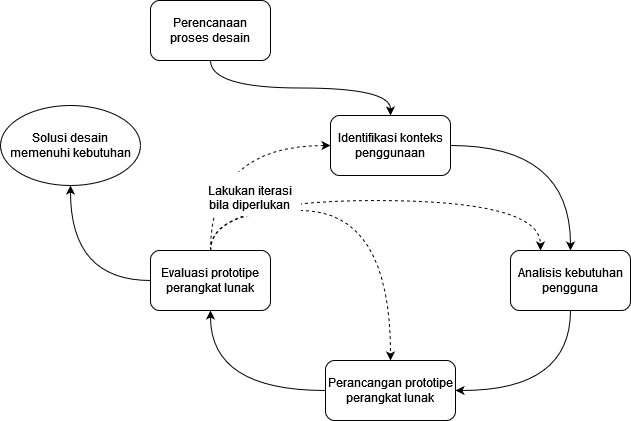
\includegraphics[width=0.8\textwidth]{chapter-1-method.png}
  \caption{Alur Kerja Penelitian}
  \label{fig:diagram_alur_kerja}
\end{figure}

\section{Perencanaan Proses Desain}
\label{sec:perencanaan_proses_desain}

Pada tahap perencanaan proses desain dilakukan persiapan sumber daya yang diperlukan selama proses desain, serta penentuan ruang lingkup permasalahan.

% Sumber daya proses design

Ruang lingkup permasalahan yang ditentukan selama pengerjaan tugas akhir sebagai berikut

\begin{enumerate}
  \item Target Pengguna
  \subitem Target pengguna selama penelitian adalah pengguna \textit{smartphone} berbasis Android di Indonesia dengan rentang umur 18-34 tahun. Rentang usia tersebut adalah usia mayoritas pengguna media sosial di Indonesia \parencite{mediasosial2020}.
  
  \item Fungsionalitas Aplikasi
  \subitem Lingkup fungsionalitas aplikasi adalah bagaimana aplikasi dapat membantu penggunanya memantau penggunaan \textit{smartphone}, membatasi waktu penggunaan aplikasi-aplikasi, serta membuat pemblokiran terjadwal terhadap akses aplikasi. Fungsionalitas lainnya menyesuaikan dengan analisis hasil yang didapatkan dari riset dan wawancara. 
  % \subitem Lingkup fungsionalitas aplikasi adalah bagaimana desain interaksi yang baru dapat memperbaiki masalah yang ditemukan pada aplikasi Digital Wellbeing saat ini. Fungsionalitas dari aplikasi menyesuaikan dengan analisis hasil yang didapatkan dari riset dan wawancara. 
   
  \item Lingkup Pengembangan Aplikasi
  \subitem Desain interaksi aplikasi pencegah distraksi yang dibuat memiliki bentuk \textit{mobile interface} dan dirancang untuk \textit{smartphone} berbasis \textit{Android}. Aplikasi Digital Wellbeing milik Google ditetapkan menjadi garis dasar pengembangan prototipe aplikasi tersebut.

\end{enumerate}

% * =======================================================================
% *   ||  ||  ||  ||  ||  ||  ||  ||  ||  ||  ||  ||  ||  ||  ||  ||  ||
% * =======================================================================

\newcommand{\ccbnormspacing}{\baselineskip=12pt}
\newcommand{\ccbnormspacingcenter}{\centering\arraybackslash\ccbnormspacing}

\section{Identifikasi Konteks Penggunaan}
\label{sec:identifikasi_konteks_penggunaan}

Pada tahap ini dilakukan proses analisis pengguna melalui data yang didapatkan dari ulasan pengguna aplikasi Digital Wellbeing dari situs Google Play Store, serta riset dengan metode wawancara. Kemudian akan dilakukan penyusunan persona pengguna dan pengidentifikasian fungsionalitas aplikasi yang akan membantu menentukan kebutuhan dan tujuan pengguna.

\subsection{Riset dan Analisis Pengguna}
\label{subsec:riset_analisis}

Tahap ini bertujuan untuk menganalis target pengguna, sehingga didapatkan data perilaku, masalah, tujuan, dan kebutuhan pengguna aplikasi Digital Wellbeing. Riset dilakukan dengan mengumpulkan data ulasan pengguna aplikasi Digital Wellbeing dari situs Google Play Store \textcite{dwplaystorereviews}. Metode pengumpulan data ini dipilih dengan alasan mengacu pada ISO 9241-210, bahwa informasi yang sudah tersedia dari suatu produk dapat dimanfaatkan untuk melakukan modifikasi atau peningkatan kualitas produk \parencite{iso9241-210:2010}, dalam hal ini informasi berbentuk ulasan pengguna.

Hasil terhadap analisis ulasan pengguna kemudian divalidasi dengan wawasan yang didapat dari wawancara. Karena pada data ulasan pengguna dari Google Play Store tidak terdapat informasi mengenai umur dan perilaku pengguna, wawancara dengan pengguna yang termasuk ke dalam lingkup permasalahan perlu dilakukan juga untuk mendapatkan wawasan mengenai perilaku pengguna. Perilaku pengguna berguna untuk menyusun persona pengguna.

\subsubsection{Ulasan Pengguna}
\label{subsubsec:ulasan_pengguna}

Berdasarkan situs Google Play Store per 13 April 2022, terdapat 609.005 ulasan untuk aplikasi Digital Wellbeing. Untuk menentukan jumlah \textit{sample size}, ditentukan \textit{confidence level} sebesar 95\%. Dikumpulkan data sebanyak 1000 ulasan dari target pengguna yang telah disebutkan pada bab \ref{sec:identifikasi_konteks_penggunaan},  kemudian dikategorikan secara manual, lalu didapatkan 288 ulasan yang dapat digunakan untuk menyusun masalah pengguna, sehingga \textit{sample} data memiliki \textit{margin of error} sebesar 5.78\%.

Pengkategorian ulasan dilakukan secara manual sehingga menghasilkan 11 kategori. Rincian tentang kategori tersebut dapat dilihat pada tabel \ref{tab:daftar_kategori}.

\newpage

\RaggedLeft
\begin{small}
\begin{longtable}[c]{|W{c}{0.08\textwidth}|>{\ccbnormspacing}m{0.72\textwidth}|>{\ccbnormspacingcenter}m{0.1\textwidth}|}
  \caption{Daftar Kategori Ulasan}
  \label{tab:daftar_kategori} \\
  \hline \rowcolor[HTML]{A3E5F5} \textbf{ID} & \centering\textbf{Kategori Ulasan} & \textbf{Jumlah Ulasan} \\ \hline \endfirsthead
  \hline \rowcolor[HTML]{A3E5F5} \textbf{ID} & \centering\textbf{Kategori Ulasan} & \textbf{Jumlah Ulasan} \\ \hline \endhead
  
  \hline \endfoot
  
  KU-01    & Kurangnya widget untuk menampilkan data di Home Screen & 63 \\ \hline
  KU-02    & Perlu dikembangkannya fitur laporan penggunaan aplikasi untuk menampilkan data & 47 \\ \hline
  KU-03    & Perlu dikembangkannya fitur Focus Mode dengan menambah keketatan & 47 \\ \hline
  KU-04    & Perlu dikembangkannya kemampuan penjadwalan untuk fitur App Timer dan Focus Mode & 36 \\ \hline
  KU-05    & Kurangnya fitur pengaturan tingkat keketatan untuk fitur-fitur & 29 \\ \hline
  KU-06    & Kurangnya kemampuan penundaan untuk fitur App Timer & 18 \\ \hline
  KU-07    & Perlu dikembangkannya fitur Bedtime Mode dengan menambah keketatan & 12 \\ \hline
  KU-08    & Kurangnya penjelasan atau susunan kata yang dapat memotivasi pengguna untuk memakai fitur-fitur aplikasi & 12 \\ \hline
  KU-09    & Kurangnya fitur pengelompokkan aplikasi & 11 \\ \hline
  KU-10    & Kurangnya fitur pengaturan jam untuk akhir sebuah hari & 7 \\ \hline
  KU-11    & Kurangnya fitur \textit{whitelisting} untuk pembatasan akses aplikasi oleh Focus Mode & 6 \\ \hline
\end{longtable}
\end{small}
\justifying
\FloatBarrier

Adapun sejumlah ulasan yang tidak tergolong dalam kategori dinilai tidak relevan dalam penyusunan masalah pengguna, dengan penjelasan sebagai berikut

\begin{enumerate}
  \item Ulasan yang menilai positif aplikasi tanpa menyebutkan adanya masalah yang ditemukan dari aplikasi
  \item Ulasan yang menilai negatif aplikasi tanpa menyebutkan masalah yang ditemukan dari aplikasi
  \item Ulasan yang menyebutkan adanya bug dari aplikasi, seperti tidak berfungsinya sebuah fitur di perangkat tertentu
  \item Ulasan yang menyebutkan masalah yang tidak termasuk ke dalam batasan tugas akhir
  \item Ulasan yang tidak dapat dimengerti, seperti huruf-huruf yang tersusun secara acak 
  \item Ulasan yang melaporkan bahwa aplikasi tidak dapat dihapus dari perangkat
\end{enumerate}

\subsubsection{Perilaku Pengguna}
Setelah melakukan analisis ulasan pengguna untuk aplikasi Digital Wellbeing, dilakukan wawancara untuk mendapatkan perilaku pengguna, memvalidasi masalah pengguna dari analisis ulasan, serta menemukan masalah lain yang tidak ditemukan dari ulasan. Target berjumlah 5 orang dengan kriteria sebagaimana telah dijelaskan pada subbab \ref{sec:perancangan_proses_desain}. Jumlah tersebut dipilih karena menurut \textcite{nielsenusabilityproblems}, penelitian dengan 5 orang responden sudah cukup untuk menemukan rata-rata 85\% masalah dari desain sebuah produk, dan menambah responden lebih banyak akan mendapatkan wawasan tambahan yang semakin sedikit.

 Data perilaku responden digunakan untuk menyusun persona pengguna, serta membantu menganalisis kebutuhan pengguna terkait aplikasi Digital Wellbeing. Sedangkan hasil validasi ulasan pengguna digunakan untuk  menggali inti masalah yang dikeluhkan. Kedua pengamatan tersebut akan dibahas lebih lanjut dalam analisis masalah, kebutuhan, dan tujuan pengguna. Rancangan pertanyaan dapat dilihat pada Lampiran \ref{chpt:daftar_pertanyaan_wawancara}. Detail pemetaan pengamatan dengan pertanyaan wawancara dapat dilihat pada Tabel \ref{tab:pemetaan_pengamatan_wawancara}

\RaggedLeft
\begin{small}
\begin{longtable}[c]{|>{\ccbnormspacing}m{0.72\textwidth}|p{0.2\textwidth}|}
  \caption{Pemetaan Pengamatan dengan Pertanyaan Wawancara}
  \label{tab:pemetaan_pengamatan_wawancara} \\
  \hline \rowcolor[HTML]{A3E5F5} \multicolumn{1}{|c|}{\textbf{Pengamatan}} & \multicolumn{1}{|c|}{\textbf{No. Pertanyaan}} \\ \hline \endfirsthead
  \hline \rowcolor[HTML]{A3E5F5} \multicolumn{1}{|c|}{\textbf{Pengamatan}} & \multicolumn{1}{|c|}{\textbf{No. Pertanyaan}} \\ \hline \endhead

  \hline \endfoot
  
  \rowcolor[HTML]{DCF3FC} \multicolumn{2}{|l|}{\textbf{A. Perilaku Responden}} \\ \hline
  Identitas responden & 1, 2, 3 \\ \hline
  Perilaku penggunaan \textit{smartphone} responden & 4, 5, 6, 7, 8 \\ \hline
  Perilaku responden terkait aplikasi pencegah distraksi & 9, 10, 11, 12 \\ \hline
  Perilaku responden terkait aplikasi \textit{Digital Wellbeing} & 13, 14, 15 \\ \hline
  \rowcolor[HTML]{DCF3FC} \multicolumn{2}{|l|}{\textbf{B. Validasi Ulasan Aplikasi Digital Wellbeing}} \\ \hline
  Validasi masalah kurangnya fitur widget pada Homescreen & 16, 17, 18 \\ \hline
  Validasi masalah pada fitur laporan data penggunaan aplikasi pada \textit{smartphone} & 19 \\ \hline
  Validasi masalah pada fitur Focus Mode & 20, 21 \\ \hline
  Validasi masalah untuk kemampuan penjadwalan pada fitur-fitur & 22, 23, 24 \\ \hline
  Validasi masalah kurangnya fitur pengaturan tingkat keketatan & 25, 26, 27 \\ \hline
  Validasi masalah kurangnya fitur penundaan pada App Timer & 28, 29, 30 \\ \hline
  Validasi masalah pada fitur Bedtime Mode & 31, 32, 33 \\ \hline
  Validasi masalah kurangnya penjelasan dan susunan kata & 34, 35 \\ \hline
  Validasi masalah kurangnya fitur pengelompokkan aplikasi & 36 \\ \hline
  Validasi masalah kurangnya fitur pengaturan jam akhir hari & 37 \\ \hline
  Validasi masalah kurangnya kemampuan \textit{whitelisting} & 38 \\ \hline
\end{longtable}
\end{small}
\justifying
\FloatBarrier

Jumlah responden yang diwawancarai adalah 10 (sepuluh) orang. Data hasil wawancara dapat dilihat pada Lampiran \ref{chpt:hasil_wawancara}. Dari 10 responden, 90\% mengakui tujuan utama dari penggunaan \textit{smartphone} adalah berkomunikasi melalui aplikasi \textit{messenger}, dengan tujuan sekunder yaitu berinteraksi dengan media sosial atau sebagai sarana hiburan. Ditemukan bahwa 4 dari 10 orang menggunakan \textit{smartphone} sebagai alat utama yang membantu dalam pekerjaan, dengan tujuan untuk berkomunikasi dengan rekan atau klien, menggunakannya sebagai \textit{workstation}, atau mencari ide dan inspirasi.

Dari wawancara, ditemukan bahwa seluruh responden mengakui distraksi terkait dengan \textit{smartphone} lebih banyak berasal dari luar \textit{smartphone} itu sendiri, yaitu dari keinginan diri sendiri menggunakan \textit{smartphone} untuk memenuhi tujuan sekunder mereka. Walaupun hanya 30\% responden yang mengeluhkan notifikasi dari \textit{smartphone} dianggap mendistraksi mereka dari kegiatan utama, 70\% mengakui perlu untuk mencegah distraksi dari notifikasi dengan cara menggunakan aplikasi pencegah distraksi atau mengubah pengaturan notifikasi aplikasinya secara langsung.

Ditemukan juga bahwa rata-rata durasi penggunaan \textit{smartphone} harian keseluruhan responden adalah 6.2 jam per hari, di mana 70\% responden dapat menggunakan \textit{smartphone} selama lebih dari 6 jam sehari. Kedua angka tersebut melebihi rata-rata durasi penggunaan \textit{smartphone} di Indonesia pada tahun 2021 yaitu 5.4 jam per hari \parencite{dataai2022smartphoneindonesia}.  Keseluruhan dari responden menilai skala rata-rata 4 (empat) dari 5 (lima) terhadap durasi penggunaan \textit{smartphone} harian mereka. Di antara seluruh responden, 70\% mengakui butuh bantuan dari sebuah aplikasi pencegah distraksi untuk menurunkan durasi penggunaan tersebut.

Selain untuk mengurangi durasi penggunaan, responden juga memerlukan bantuan sebuah aplikasi untuk melakukan hal lain yang berhubungan dengan perbaikan kebiasaan digital mereka. Ditemukan 50\% responden memerlukan bantuan aplikasi untuk memantau penggunaan \textit{smartphone}, baik secara keseluruhan atau per aplikasi, dalam merencanakan perbaikan digital mereka. Lalu, 80\% dari responden merasa perlu diingatkan tentang tugas / kegiatan yang harus diselesaikan saat mereka menggunakan \textit{smartphone}. Keberadaan sebuah pengingat dapat menyadarkan pengguna terhadap alasan mereka menggunakan aplikasi pencegah distraksi. Selain itu, 50\% dari responden juga menggunakan aplikasi untuk membantu dalam memperbaiki jadwal tidurnya. Mereka mengakui bahwa saat menggunakan \textit{smartphone} sebelum tidur, seringkali mereka tidak menyadari waktu sehingga melewati jadwal tidur mereka.

Wawasan tentang perilaku pengguna yang didapat dapat disusun dalam bentuk variabel-variabel perilaku yang berguna dalam pembentukan persona. \textcite{cooper2014face} menyarankan bahwa dalam menyusun variabel dapat ditemukan perbedaan yang cukup jelas jika fokus kepada tipe-tipe variabel berikut
\begin{enumerate}
  \item Aktivitas, yaitu apa yang dilakukan pengguna dan seberapa sering 
  \item Sikap, yaitu pendapat pengguna tentang domain produk dan teknologi
  \item Kemampuan, yaitu bakat pengguna dan kemampuan untuk belajar
  \item Motivasi, yaitu alasan keterlibatan pengguna pada domain produk 
  \item Keterampilan, yaitu kemampuan pengguna terkait domain produk dan teknologi
\end{enumerate}

Keseluruhan variabel perilaku pengguna dirangkum pada Tabel \ref{tab:perilaku_pengguna}

\newpage

\RaggedLeft
\begin{small}
\begin{longtable}[c]{|W{c}{0.07\textwidth}|>{\ccbnormspacing}m{0.66\textwidth}|>{\ccbnormspacingcenter}m{0.165\textwidth}|}
  \caption{Daftar Variabel Perilaku Pengguna}
  \label{tab:perilaku_pengguna} \\
  \hline \rowcolor[HTML]{A3E5F5} \textbf{ID} & \multicolumn{1}{|c|}{\textbf{Variabel Perilaku Pengguna}} & \multicolumn{1}{|c|}{\textbf{Tipe Perilaku}} \\ \hline \endfirsthead
  \hline \rowcolor[HTML]{A3E5F5} \textbf{ID} & \multicolumn{1}{|c|}{\textbf{Variabel Perilaku Pengguna}} & \multicolumn{1}{|c|}{\textbf{Tipe Perilaku}} \\ \hline \endhead
  
  \hline \endfoot
  
  PP-01  &  Menggunakan \textit{smartphone} dengan tujuan primer untuk berkomunikasi melalui aplikasi \textit{messenger}  & Aktivitas \\ \hline
  PP-02  &  Menggunakan \textit{smartphone} dengan tujuan primer untuk membantu dalam pekerjaan & Aktivitas \\ \hline
  PP-03  &  Menggunakan \textit{smartphone} dengan tujuan sekunder untuk berinteraksi lewat media sosial & Aktivitas \\ \hline
  PP-04  &  Menggunakan \textit{smartphone} dengan tujuan sekunder sebagai sarana hiburan & Aktivitas \\ \hline
  PP-05  &  Menilai skala rata-rata 4 (empat) dari 5 (lima) terhadap durasi penggunaaan \textit{smartphone} harian & Aktivitas \\ \hline
  PP-06  &  Merasa sering terdistraksi oleh keinginan diri sendiri untuk menggunakan \textit{smartphone}  & Sikap \\ \hline
  PP-07  &  Merasa sering terdistraksi oleh notifikasi dari \textit{smartphone} & Sikap \\ \hline
  PP-08  &  Merasa \textit{smartphone} sebaiknya membatasi pengguna seminimal mungkin & Sikap \\ \hline
  PP-09  &  Merasa perlu ada sebuah penghargaan jika berhasil mengikuti jadwal pembatasan \textit{smartphone} & Sikap \\ \hline
  PP-10  &  Mampu membatasi diri dari menggunakan \textit{smartphone} tanpa bantuan & Kemampuan \\ \hline
  PP-11  &  Ingin memblokir notifikasi aplikasi yang dinilai sebagai distraksi & Motivasi \\ \hline
  PP-12  &  Ingin mengurangi durasi penggunaan \textit{smartphone} harian & Motivasi \\ \hline
  PP-13  &  Ingin memantau kebiasaan penggunaan \textit{smartphone} & Motivasi \\ \hline
  PP-14  &  Ingin dibantu mengingatkan diri terhadap tugas / aktivitas yang harus dilakukan & Motivasi \\ \hline
  PP-15  &  Ingin mengingatkan diri terhadap jadwal tidur & Motivasi \\ \hline
  PP-16  &  Ingin diingatkan ketika terlalu lama menggunakan aplikasi & Motivasi \\ \hline
  PP-17  &  Ingin memblokir akses ke aplikasi yang dinilai mendistraksi tanpa menghapusnya & Motivasi \\ \hline
  PP-18  &  Mampu mengatur jadwal kegiatan dengan baik sehingga tidak mudah terdistraksi & Keterampilan \\ \hline
  PP-19  &  Terbiasa dalam mengoperasikan aplikasi pencegah distraksi pada \textit{smartphone}  & Keterampilan \\ \hline
\end{longtable}
\end{small}
\justifying
\FloatBarrier

\subsubsection{Masalah Pengguna}
\label{subsubsec:masalah_pengguna}

Ditemukan bahwa kategori ulasan yang didapat dari analisis ulasan pengguna cukup bervariasi dengan jumlah yang tersebar. Namun, ulasan pengguna tidak cukup dalam menggambarkan inti dari masalah yang mereka alami. Tahap verifikasi dari wawancara membantu menemukan inti masalah yang dikeluhkan serta gambaran utama dari keseluruhan masalah tersebut. Pengguna mengeluhkan bahwa mereka kurang dapat mendapat gambaran tentang kebiasaan digital yang baik dari aplikasi Digital Wellbeing. Selain itu, pengguna juga kesulitan dalam menggunakan aplikasi Digital Wellbeing secara efisien untuk mencapai tujuan-tujuannya.

Untuk menyelesaikannya, masalah tersebut perlu dipecahkan menjadi masalah-masalah pengguna yang dapat dirincikan. Hal tersebut dilakukan untuk mempermudah penentuan kebutuhan dan tujuan pengguna serta penyusunan solusi. Keseluruhan masalah pengguna dirangkum pada Tabel \ref{tab:daftar_masalah}.

\RaggedLeft
\begin{small}
\begin{longtable}[c]{|W{c}{0.08\textwidth}|>{\ccbnormspacing}m{0.6\textwidth}|>{\ccbnormspacingcenter}m{0.2\textwidth}|}
  \caption{Daftar Masalah Pengguna}
  \label{tab:daftar_masalah} \\
  \hline \rowcolor[HTML]{A3E5F5}
  \textbf{ID} & \centering\textbf{Masalah Pengguna} & \textbf{Keterkaitan} \\ \hline \endfirsthead
  \hline \rowcolor[HTML]{A3E5F5}
  \textbf{ID} & \centering\textbf{Masalah Pengguna} & \textbf{Keterkaitan} \\ \hline \endhead

  \hline \endfoot

  MP-01  & Pengguna kesulitan dalam melakukan pengaturan fitur-fitur aplikasi Digital Wellbeing secara efisien & KU-01, KU-04, KU-05, KU-09, KU-10, KU-11 \\ \hline
  MP-02  & Pengguna kesulitan dalam menganalisis kebiasaan digital diri lewat aplikasi Digital Wellbeing & KU-02 \\ \hline
  MP-03  & Pengguna merasa fitur-fitur aplikasi Digital Wellbeing kurang ketat dalam membantu memperbaiki kebiasaan digital & KU-03, KU-04, KU-05, KU-06, KU-07 \\ \hline
  MP-04  & Pengguna merasa fitur-fitur aplikasi Digital Wellbeing kurang fleksibel & KU-04, KU-06, KU-09, KU-10 \\ \hline
  MP-05  & Pengguna merasa interaksi dengan aplikasi Digital Wellbeing kurang pribadi & KU-08 \\ \hline
  MP-06  & Pengguna kurang dapat memahami penggunaan fitur-fitur yang disediakan oleh aplikasi Digital Wellbeing & KU-08 \\ \hline
  MP-07  & Pengguna kesulitan dalam mengakses informasi pada fitur-fitur aplikasi Digital Wellbeing & KU-01 \\ \hline
\end{longtable}
\end{small}
\justifying
\FloatBarrier

% $ =====================================================
% $   +  +  +  +  +  +  +  +  +  +  +  +  +  +  +  +  +
% $ =====================================================


\subsection{Persona}
\label{subsec:persona_pengguna}
Setelah dilakukan analisis mengenai perilaku dan masalah pengguna, dilakukan segmentasi pengguna menjadi beberapa kelompok persona. Persona merepresentasikan kelompok-kelompok pengguna dengan karakteristik dan perilaku yang berbeda. Persona berperan menjadi arah pengembangan interaksi aplikasi dan mengurangi kemungkinan mendesain aplikasi untuk semua orang sehingga menghasilkan desain yang tidak disenangi oleh siapapun. \parencite{cooper2014face}

\subsubsection{Pengelompokkan Awal Pengguna}
Tahap awal dalam menyusun persona adalah mengelompokkan pengguna-pengguna berdasarkan perannya. Dari 10 orang partisipan riset wawancara, dikelompokkan menjadi 3 peran berdasarkan kemampuannya dalam membatasi diri dari \textit{smartphone} tanpa membutuhkan bantuan, dengan kata lain kemampuan penguasaan diri mereka. Kemampuan ini dianalisis dari data-data yang didapat melalui wawancara, semakin tinggi tingkat kemampuannya berarti pengguna tersebut dapat membatasi dirinya dengan bantuan sesedikit mungkin.

Terdapat pengguna dengan kemampuan penguasaan diri tingkat rendah beranggotakan 20\% partisipan, pengguna berkemampuan tingkat sedang sebanyak 30\%, dan pengguna dengan kemampuan tingkat tinggi sebanyak 50\%. Maka dari itu, pembagian untuk kelompok pengguna adalah sebagai berikut\begin{enumerate}
  \item Kelompok 1: Pengguna yang sangat memerlukan bantuan untuk membatasi diri dari \textit{smartphone} 
  \item Kelompok 2: Pengguna yang memerlukan bantuan ringan untuk membatasi diri dari \textit{smartphone}
  \item Kelompok 3: Pengguna yang tidak memerlukan bantuan untuk membatasi diri dari \textit{smartphone}
\end{enumerate}

\subsubsection{Pemetaan Kelompok Pengguna dengan Variabel Perilaku}
Setelah dilakukan pengelompokkan pengguna, variabel-variabel perilaku yang telah diidentifikasi pada tahap riset dan analisis pengguna perlu dipetakan ke setiap kelompok pengguna. Hal ini bertujuan untuk mengidentifikasi perilaku dari setiap kelompok untuk kemudian disusun personanya.

Variabel perilaku yang dipetakan ke masing-masing kelompok pengguna akan memiliki jenis nilai yang berbeda. Variabel perilaku seperti PP-01 dan PP-02 menunjukkan apa saja nilai perilaku yang dipenuhi kelompok pengguna tersebut. Variabel perilaku seperti PP-10 dan PP-19 menunjukkan rentang atau tingkat perilaku dari kelompok pengguna tersebut. Sedangkan variabel perilaku seperti PP-08 dan PP-09 menunjukkan apakah pengguna memiliki perilaku tersebut. Hasil dari proses pemetaan dapat dilihat pada Tabel \ref{tab:pemetaan_perilaku}.

\RaggedLeft
\begin{small}
\begin{longtable}[c]{|>{\ccbnormspacing}m{0.10\textwidth}|>{\ccbnormspacing}m{0.31\textwidth}|>{\ccbnormspacingcenter}m{0.145\textwidth}|>{\ccbnormspacingcenter}m{0.145\textwidth}|>{\ccbnormspacingcenter}m{0.145\textwidth}|}
  \caption{Daftar Pemetaan Kelompok Pengguna dengan Variabel Perilaku}
  \label{tab:pemetaan_perilaku} \\
  \hline \rowcolor[HTML]{A3E5F5}
  \centering\textbf{Variabel Perilaku} & \centering\textbf{Deskripsi Perilaku} & \textbf{Kelompok 1} & \textbf{Kelompok 2} & \textbf{Kelompok 3} \\ \hline \endfirsthead
  \hline \rowcolor[HTML]{A3E5F5}
  \centering\textbf{Variabel Perilaku} & \centering\textbf{Deskripsi Perilaku} & \textbf{Kelompok 1} & \textbf{Kelompok 2} & \textbf{Kelompok 3} \\ \hline \endhead

  \hline \endfoot

  \centering PP-10  & Mampu membatasi diri dari menggunakan \textit{smartphone} tanpa bantuan & Rendah & Sedang & Tinggi \\ \hline
  \centering PP-01 PP-02  & Tujuan primer menggunakan \textit{smartphone} & Komunikasi & Pekerjaan, Komunikasi & Komunikasi, Pekerjaan \\ \hline
  \centering PP-03 PP-04 & Tujuan sekunder menggunakan \textit{smartphone} & Hiburan, Media sosial & Hiburan, Media sosial & Hiburan, Media sosial \\ \hline
  \centering PP-05 & Penilaian durasi penggunaan \textit{smartphone} harian berdasarkan skala 1-5 & 5 & 4 & 3 \\ \hline
  \centering PP-06 PP-07 & Sumber distraksi terkait \textit{smartphone} & Keinginan diri sendiri, \textit{smartphone}, pihak lain & Keinginan diri sendiri, \textit{smartphone}, pihak lain & Keinginan diri sendiri \\ \hline
  \centering PP-18 & Keterampilan dalam menyusun jadwal kegiatan & Rendah & Tinggi & Sedang \\ \hline
  \centering PP-19 & Kebiasaan dalam menggunakan aplikasi pencegah distraksi & Tinggi & Sedang & Sedang \\ \hline
  \centering PP-08 & Merasa \textit{smartphone} sebaiknya membatasi pengguna seminimal mungkin &   & \textbf{V} & \textbf{V} \\ \hline
  \centering PP-09 & Merasa perlu ada sebuah penghargaan jika berhasil mengikuti jadwal pembatasan \textit{smartphone} & \textbf{V} &   &   \\ \hline
  \centering PP-11 & Ingin memblokir notifikasi aplikasi yang dinilai sebagai distraksi & \textbf{V} & \textbf{V} & \textbf{V} \\ \hline
  \centering PP-12 & Ingin mengurangi durasi penggunaan \textit{smartphone} harian & \textbf{V} & \textbf{V} & \textbf{V} \\ \hline
  \centering PP-13 & Ingin memantau kebiasaan penggunaan \textit{smartphone} & \textbf{V} & \textbf{V} & \textbf{V} \\ \hline
  \centering PP-14 & Ingin dibantu mengingatkan diri terhadap tugas / aktivitas yang harus dilakukan & \textbf{V} & \textbf{V} &   \\ \hline
  \centering PP-15 & Ingin mengingatkan diri terhadap jadwal tidur & \textbf{V} & \textbf{V} &   \\ \hline
  \centering PP-16 & Ingin diingatkan ketika terlalu lama menggunakan aplikasi & \textbf{V} &   &   \\ \hline
  \centering PP-17 & Ingin memblokir akses ke aplikasi yang dinilai mendistraksi tanpa menghapusnya & \textbf{V} &   &   \\ \hline

\end{longtable}
\end{small}
\justifying
\FloatBarrier

\subsubsection{Pemetaan Kelompok Pengguna dengan Masalah Pengguna}
Selain variabel perilaku, masalah pengguna pun perlu dipetakan dengan kelompok pengguna yang telah dibuat. Hal ini dilakukan untuk mengenali masalah yang dirasakan oleh kelompok pengguna spesifik, dan juga membantu dalam menyusun persona.

Ditemukan bahwa ketiga kelompok pengguna mengalami sebagian besar dari masalah pengguna yang ada. Masalah pengguna MP-03 di mana aplikasi Digital Wellbeing dinilai kurang ketat tidak dirasakan oleh kelompok pengguna 3 karena tingginya kemampuan dalam membatasi diri dari \textit{smartphone} tanpa membutuhkan bantuan. Di sisi lain, masalah MP-04 tentang fleksibilitas aplikasi tidak dirasakan oleh kelompok pengguna 1 dengan tingkat penguasaan diri yang rendah dan kebutuhan mereka atas bantuan yang ketat untuk membatasi penggunaan \textit{smartphone}. Selain itu, akibat keterampilan kelompok pengguna 1 dalam menggunakan aplikasi pencegah distraksi, mereka tidak mengalami masalah MP-06 karena mereka sudah cukup mengerti fitur-fitur yang digunakan. Hasil dari proses pemetaan dapat dilihat pada Tabel \ref{tab:pemetaan_masalah}.

\RaggedLeft
\begin{small}
\begin{longtable}[c]{|>{\ccbnormspacing}m{0.08\textwidth}|>{\ccbnormspacing}m{0.31\textwidth}|>{\ccbnormspacingcenter}m{0.145\textwidth}|>{\ccbnormspacingcenter}m{0.145\textwidth}|>{\ccbnormspacingcenter}m{0.145\textwidth}|}
  \caption{Daftar Pemetaan Kelompok Pengguna dengan Masalah Pengguna}
  \label{tab:pemetaan_masalah} \\
  \hline \rowcolor[HTML]{A3E5F5}
  \centering\textbf{ID} & \centering\textbf{Deskripsi Masalah} & \textbf{Kelompok 1} & \textbf{Kelompok 2} & \textbf{Kelompok 3} \\ \hline \endfirsthead
  \hline \rowcolor[HTML]{A3E5F5}
  \centering\textbf{ID} & \centering\textbf{Deskripsi Masalah} & \textbf{Kelompok 1} & \textbf{Kelompok 2} & \textbf{Kelompok 3} \\ \hline \endhead

  \hline \endfoot

  \centering MP-01 & Pengguna kesulitan dalam melakukan pengaturan fitur-fitur aplikasi Digital Wellbeing secara efisien & \textbf{V} & \textbf{V} & \textbf{V} \\ \hline
  \centering MP-02 & Pengguna kesulitan dalam menganalisis kebiasaan digital diri lewat aplikasi Digital Wellbeing & \textbf{V} & \textbf{V} & \textbf{V} \\ \hline
  \centering MP-03 & Pengguna merasa fitur-fitur aplikasi Digital Wellbeing kurang ketat dalam membantu memperbaiki kebiasaan digital & \textbf{V} & \textbf{V} &  \\ \hline
  \centering MP-04 & Pengguna merasa fungsionalitas fitur-fitur aplikasi Digital Wellbeing kurang fleksibel &  & \textbf{V} & \textbf{V} \\ \hline
  \centering MP-05 & Pengguna merasa interaksi dengan aplikasi Digital Wellbeing kurang pribadi & \textbf{V} & \textbf{V} & \textbf{V} \\ \hline
  \centering MP-06 & Pengguna kurang dapat memahami penggunaan fitur-fitur yang disediakan oleh aplikasi Digital Wellbeing &  & \textbf{V} & \textbf{V} \\ \hline
  \centering MP-07 & Pengguna kesulitan dalam mengakses informasi pada fitur-fitur aplikasi Digital Wellbeing & \textbf{V} & \textbf{V} & \textbf{V} \\ \hline

\end{longtable}
\end{small}
\justifying
\FloatBarrier

\subsubsection{Penyusunan Karakteristik Persona}
Setelah dilakukan pemetaan kelompok pengguna terhadap variabel perilaku dan masalah, kelompok pengguna tersebut dapat disusun menjadi persona yang utuh dengan diberikan identitas dan karakter dalam bentuk sebuah narasi. Di dalam narasi tersebut, garis besar hasil pemetaan juga perlu disebutkan ulang. Hal-hal tersebut dapat membuat persona terasa hidup sehingga mempermudah proses penentuan kebutuhan dan tujuan pengguna, serta pembuatan solusi desain.

Berikut adalah hasil penyusunan karakteristik persona untuk ketiga kelompok pengguna

\begin{enumerate}
  \item Persona 1: Nico
  \subitem Nico adalah seorang mahasiswa berumur 21 tahun yang sedang menjalani semester akhir di universitasnya. Nico mengerjakan tugas akhir pada laptopnya, namun ia merasa mudah terdistraksi oleh \textit{smartphone}nya, baik dari keinginannya untuk memeriksa media sosial atau permainan, maupun notifikasi yang sering muncul. Oleh karena itu, Nico menggunakan aplikasi Digital Wellbeing untuk memblokir akses ke aplikasi yang ia rasa mendistraksi serta mematikan notifikasinya. Namun terkadang Nico membuka blokirnya terlalu sering sehingga dia merasa adanya fitur dari Digital Wellbeing tidak berpengaruh dalam membantunya mencegah distraksi dari \textit{smartphone}-nya. Nico merasa butuh bantuan yang cukup besar dalam mengendalikan dirinya terkait \textit{smartphone} karena ia sering menyadari bahwa dirinya terlalu sering menggunakan \textit{smartphone}, melupakan tugasnya, dan jadwal tidurnya pun terganggu.

  \item Persona 2: Maya
  \subitem Maya adalah seorang pegawai swasta berumur 28 tahun. Dalam kesehariannya, Maya menggunakan \textit{smartphone} untuk berkomunikasi dengan rekan kerjanya, membantu dalam pekerjaannya, dan sebagai hiburan di jam istirahat. Maya sering terdistraksi di jam kerjanya oleh notifikasi atau keinginannya untuk memeriksa \textit{smartphone}, sehingga menggunakan aplikasi Digital Wellbeing untuk memblokirnya. Maya menemukan fitur-fitur menarik lain yang ia rasa dapat membantu mencegah distraksi, dan menganalisa serta memperbaiki kebiasaan penggunaan \textit{smartphone}nya. Namun Maya merasa bahwa beberapa fitur dari Digital Wellbeing kurang fleksibel untuk menyesuaikan dengan jadwal kerjanya yang bervariasi, seperti kurangnya kemampuan membuat jadwal lebih dari satu. Maya juga merasa pengalaman yang dirasakan kurang cukup personal untuk cukup memotivasinya karena pesan pengingat yang ia dapatkan terlalu membosankan.

  \item Persona 3: Nathan
  \subitem Nathan adalah seorang lulusan baru dan pekerja yang berumur 23 tahun. Dia terbiasa dalam mengatur jadwal pekerjaannya, dan sesekali menyelipkan jadwal untuk beristirahat. Ia melakukan sebagian besar pekerjaannya menggunakan \textit{smartphone}, seperti berkomunikasi, mengatur jadwal, dan menulis catatan. Nathan sesekali merasa bahwa dirinya memeriksa media sosial di \textit{smartphone} di waktu yang tidak tepat di saat jadwal kerjanya. Maka Nathan menggunakan fitur Focus Mode dari Digital Wellbeing untuk mengingatkan dirinya jika akan bermain \textit{smartphone} di jam kerjanya dan memblokir notifikasi dari aplikasi-aplikasi yang dianggap mendistraksi. Namun, Nathan tidak menggunakan fitur lain dari Digital Wellbeing karena ia merasa tidak perlu bantuan cukup banyak, tampilan dari aplikasi tidak cukup menarik, dan fitur-fitur yang ada tidak memiliki deskripsi yang jelas atau pengaturan yang cukup mudah.

\end{enumerate}

\subsubsection{Pemilihan Tipe Persona}
Dari persona-persona yang telah disusun, perlu dipilih sebuah persona primer. Persona primer akan dijadikan target utama atau panduan dalam membuat desain solusi. Persona primer yang dipilih harus dipertimbangkan agar tidak mengecewakan persona-persona lainnya. Dalam hal ini, persona 2, Maya, akan dijadikan sebagai persona primer. Namun dipilih juga persona 1, Nico, sebagai persona sekunder agar desain solusi yang dibuat tetap mampu memenuhi kebutuhannya.

\newpage
Keputusan ini diambil melihat pertimbangan bahwa salah satu masalah terbesar dari aplikasi Digital Wellbeing adalah sulitnya pengguna dalam menggunakan aplikasi secara efisien untuk mencapai tujuan-tujuannya. Masalah tersebut tercerminkan dari masalah-masalah yang dikeluhkan oleh persona Maya dan persona lainnya. Dalam hal itu, solusi yang didesain untuk persona Maya diharapkan dapat menyelesaikan masalah-masalah yang dialami persona lain. Di sisi lain, kemampuan penguasaan diri dari persona Nico perlu dipertimbangkan dalam solusi desain, tanpa mengganggu desain yang ditujukan untuk persona primer.

% $ =====================================================
% $   +  +  +  +  +  +  +  +  +  +  +  +  +  +  +  +  +
% $ =====================================================


\subsection{Analisis Fungsionalitas Aplikasi}
\label{subsec:analisis_fungsionalitas}

Dalam mengidentifikasi konteks penggunaan produk, penting untuk mengerti lingkungan sistem dari produk tersebut untuk membantu mengidentifikasi kebutuhan pengguna. Untuk Tugas Akhir ini, perlu diidentifikasi fungsionalitas dari aplikasi Digital Wellbeing, yang dilakukan dengan mengobservasi aplikasinya langsung, serta fungsionalitas dari aplikasi pencegah distraksi pada umumnya. Dalam Tabel \ref{tab:daftar_fungsionalitas_app_dw} terdapat fungsionalitas dari aplikasi Digital Wellbeing yang sudah diterapkan, sedangkan dalam Tabel \ref{tab:daftar_fungsionalitas_app_umum} terdapat fungsionalitas dari aplikasi-aplikasi pencegah distraksi pada umumnya dengan mengacu pada penelitian yang telah dipelajari sebagai bagian dari studi literatur Bab \ref{sec:penelitian_terkait}.

\RaggedLeft
\begin{small}
\begin{longtable}[c]{|W{c}{0.08\textwidth}|>{\ccbnormspacing}m{0.82\textwidth}|}
  \caption{Daftar Fungsionalitas Aplikasi Digital Wellbeing}
  \label{tab:daftar_fungsionalitas_app_dw} \\
  \hline \rowcolor[HTML]{A3E5F5} \textbf{ID} & \multicolumn{1}{|c|}{\textbf{Fungsionalitas Digital Wellbeing}} \\ \hline \endfirsthead
  \hline \rowcolor[HTML]{A3E5F5} \textbf{ID} & \multicolumn{1}{|c|}{\textbf{Fungsionalitas Digital Wellbeing}} \\ \hline \endhead
  
  \hline \endfoot
  
  FD-01  &  Aplikasi dapat melacak penggunaan harian \textit{smartphone} dari sisi durasi penggunaan, jumlah pembukaan, dan notifikasi yang diterima \\ \hline
  FD-02  &  Aplikasi dapat melacak penggunaan harian aplikasi-aplikasi, dari sisi durasi penggunaan, jumlah pembukaan, dan notifikasi yang dikirim \\ \hline
  FD-03  &  Aplikasi dapat menampilkan laporan penggunaan \textit{smartphone} atau aplikasi-aplikasi dalam bentuk grafik \\ \hline
  FD-04  &  Aplikasi dapat menampilkan laporan penggunaan \textit{smartphone} atau aplikasi-aplikasi dalam bentuk daftar \\ \hline
  FD-05  &  Pengguna dapat mengatur batas waktu per hari akses suatu aplikasi \\ \hline
  FD-06  &  Aplikasi dapat memberikan notifikasi terkait batas waktu akses suatu aplikasi \\ \hline
  FD-07  &  Aplikasi dapat memunculkan jendela pengingat batas waktu akses aplikasi \\ \hline
  FD-08  &  Aplikasi dapat memblokir akses terhadap suatu aplikasi \\ \hline
  FD-09  &  Aplikasi dapat memblokir notifikasi yang dikirim suatu aplikasi \\ \hline
  FD-10  &  Pengguna dapat mengatur jadwal aktivasi pemblokiran akses aplikasi \\ \hline
  FD-11  &  Pengguna dapat menunda pemblokiran akses sebuah aplikasi secara sementara \\ \hline
  FD-12  &  Pengguna dapat mengatur jadwal aktivasi mode waktu tidur \textit{smartphone} \\ \hline
  FD-13  &  Pengguna dapat menunda sementara aktivasi mode waktu tidur \textit{smartphone} \\ \hline
  FD-14  &  Pengguna dapat membuka pengaturan notifikasi aplikasi \\ \hline
  FD-15  &  Aplikasi dapat mengubah warna layar menjadi hitam-putih \\ \hline
\end{longtable}
\end{small}
\justifying
\FloatBarrier

\RaggedLeft
\begin{small}
\begin{longtable}[c]{|W{c}{0.08\textwidth}|>{\ccbnormspacing}m{0.82\textwidth}|}
  \caption{Daftar Fungsionalitas Aplikasi Pencegah Distraksi Pada Umumnya}
  \label{tab:daftar_fungsionalitas_app_umum} \\
  \hline \rowcolor[HTML]{A3E5F5} \textbf{ID} & \multicolumn{1}{|c|}{\textbf{Fungsionalitas Umum}} \\ \hline \endfirsthead
  \hline \rowcolor[HTML]{A3E5F5} \textbf{ID} & \multicolumn{1}{|c|}{\textbf{Fungsionalitas Umum}} \\ \hline \endhead
  
  \hline \endfoot
  
  FU-01  &  Aplikasi dapat melacak penggunaan harian \textit{smartphone}, dari sisi durasi penggunaan dan jumlah pembukaan \\ \hline
  FU-02  &  Aplikasi dapat melacak penggunaan harian aplikasi-aplikasi, dari sisi durasi penggunaan dan jumlah pembukaan \\ \hline
  FU-03  &  Aplikasi dapat mempresentasikan data penggunaan \textit{smartphone} harian berupa ringkasan pemakaian \textit{smartphone} dan aplikasi-aplikasi \\ \hline
  FU-04  &  Aplikasi dapat menampilkan data penggunaan \textit{smartphone} dalam bentuk grafik \\ \hline
  FU-05  &  Aplikasi dapat menampilkan data penggunaan \textit{smartphone} dalam bentuk daftar \\ \hline
  FU-06  &  Aplikasi dapat menampilkan data penggunaan \textit{smartphone} dalam sebuah \textit{widget} \\ \hline
  FU-07  &  Aplikasi dapat menampilkan data penggunaan \textit{smartphone} dalam sebuah notifikasi \\ \hline
  FU-08  &  Pengguna dapat mengatur batas waktu per hari akses \textit{smartphone} \\ \hline
  FU-09  &  Pengguna dapat mengatur pemblokiran terhadap akses \textit{smartphone} untuk durasi waktu yang ditentukan \\ \hline
  FU-10  &  Pengguna dapat mengheningkan suara dari \textit{smartphone} dan menguncinya untuk waktu yang ditentukan \\ \hline
  FU-11  &  Pengguna dapat mengatur batas waktu per hari akses suatu aplikasi \\ \hline
  FU-12  &  Pengguna dapat mengatur pemblokiran terhadap suatu aplikasi untuk durasi waktu yang ditentukan \\ \hline
  FU-13  &  Pengguna dapat memasang pemblokiran terhadap \textit{smartphone} atau suatu aplikasi jika memenuhi konteks penggunaan yang diatur pengguna, seperti saat melakukan aktivitas, atau di lokasi tertentu \\ \hline
  FU-14  &  Pengguna dapat menunda pemblokiran akses \textit{smartphone} secara sementara \\ \hline
  FU-15  &  Pengguna dapat menghapus pemblokiran akses \textit{smartphone}\\ \hline
  FU-16  &  Pengguna dapat menunda pemblokiran akses sebuah aplikasi secara sementara \\ \hline
  FU-17  &  Pengguna dapat menghapus pemblokiran akses sebuah aplikasi \\ \hline
  FU-18  &  Aplikasi dapat memunculkan jendela pengingat batas waktu penggunaan \textit{smartphone} atau aplikasi \\ \hline
  
  
\end{longtable}
\end{small}
\justifying
\FloatBarrier

\subsection{Analisis Kebutuhan dan Tujuan Pengguna}
\label{subsec:analisis_kebutuhan_tujuan}

Bagian dari identifikasi konteks penggunaan ini akan menganalisis tentang kebutuhan serta tujuan dari pengguna mengenai aplikasi Digital Wellbeing dan aplikasi pencegah distraksi secara umum, dibantu dengan data dari perilaku dan persona pengguna, masalah pengguna, dan fungsionalitas aplikasi. Keduanya akan berguna dalam merancang perbaikan desain interaksi yang diperlukan dari aplikasi Digital Wellbeing, terutama untuk menyusun \textit{usability} dan \textit{user experience goals}.

\subsubsection{Kebutuhan Pengguna}
\label{subsubsec:kebutuhan_pengguna}

Kebutuhan pengguna adalah hal apa saja yang diperlukan pengguna untuk mencapai tujuannya dalam memakai aplikasi Digital Wellbeing. Analisis kebutuhan pengguna melibatkan masalah pengguna serta perilaku pengguna yang telah dibahas sebelumnya. Penjelasan kebutuhan pengguna dirangkum di dalam Tabel \ref{tab:daftar_kebutuhan}.

\RaggedLeft
\begin{small}
\begin{longtable}[c]{|W{c}{0.07\textwidth}|>{\ccbnormspacing}m{0.65\textwidth}|>{\ccbnormspacingcenter}m{0.19\textwidth}|}
  \caption{Daftar Kebutuhan Pengguna}
  \label{tab:daftar_kebutuhan} \\
  \hline \rowcolor[HTML]{A3E5F5}
  \textbf{ID} & \centering\textbf{Kebutuhan Pengguna} & \textbf{Keterkaitan} \\ \hline \endfirsthead
  \hline \rowcolor[HTML]{A3E5F5}
  \textbf{ID} & \centering\textbf{Kebutuhan Pengguna} & \textbf{Keterkaitan} \\ \hline \endhead

  \hline \endfoot

  KP-01  & Pengalaman pengaturan fitur yang lebih efisien dengan kemampuan seperti pencarian dan pengelompokan aplikasi & MP-01, PP-18, PP-19 \\ \hline
  KP-02  & Widget untuk mengakses data serta melakukan pengaturan terhadap fitur-fitur lewat Homescreen & MP-01, MP-02, MP-07, PP-13, PP-19 \\ \hline
  KP-03  & Fitur rekomendasi untuk memberikan informasi tentang kebiasaan digital yang baik dan aksi yang dapat dilakukan & MP-02, MP-05, PP-12, PP-13 \\ \hline
  KP-04  & Laporan penggunaan \textit{smartphone} dengan rentang waktu lebih banyak dan ringkasan informasi seperti rata-rata penggunaan & MP-02, PP-13 \\ \hline
  KP-05  & Pengaturan tingkat keketatan untuk kemampuan tertentu dari fitur-fitur & MP-03, PP-08, PP-10 \\ \hline
  KP-06  & Kemampuan penguncian pengaturan untuk mencegah pengubahan oleh pengguna & MP-03, PP-06, PP-08, PP-10 \\ \hline
  KP-07  & Fitur penjadwalan dengan kemampuan menambah lebih dari satu jadwal aktivasi fitur & MP-04, PP-18  \\ \hline
  KP-08  & Kemampuan penundaan pada restriksi yang diterapkan oleh fitur-fitur & MP-04, PP-08 \\ \hline
  KP-09  & Kemampuan pengaturan pesan untuk melakukan personalisasi pesan-pesan pengingat dari fitur-fitur & MP-05, PP-09, PP-14 \\ \hline
  KP-10  & Tampilan aplikasi yang lebih menarik dengan deskripsi fitur yang lebih jelas & MP-06, PP-19 \\ \hline
  KP-11  & Fitur penghargaan jika berhasil mencapai target yang dipasang atau mengurangi waktu penggunaan \textit{smartphone} & MP-05, PP-09 \\ \hline
\end{longtable}
\end{small}
\justifying
\FloatBarrier

\subsubsection{Tujuan dan Kegiatan Pengguna}
\label{subsubsec:tujuan_kegiatan_pengguna}

Dengan ditentukannya kebutuhan pengguna, maka dapat dianalisis tujuan yang ingin dicapai oleh pengguna. Dalam mencapai tujuan-tujuan tersebut, maka perlu ditentukan kegiatan yang harus dilakukan oleh pengguna, atau disebut sebagai \textit{user task}. Analisis tujuan dan kegiatan pengguna dilakukan dengan mengkaitkan kebutuhan pengguna dan perilaku pengguna. Hasil analisis dirangkum pada Tabel \ref{tab:daftar_tujuan_kegiatan}.

\newlength{\cccolid}
\setlength{\cccolid}{0.09\textwidth}

\newlength{\cccolgoal}
\setlength{\cccolgoal}{0.2\textwidth}

\newlength{\cccolneed}
\setlength{\cccolneed}{0.14\textwidth}

\newcommand{\ccid}[2]{\multirow{#1}{\cccolid}{\centering\linespread{1}\selectfont #2}}
\newcommand{\ccgoal}[2]{\multirow{#1}{\cccolgoal}{\linespread{1}\selectfont #2}}
\newcommand{\ccneed}[2]{\multirow{#1}{\cccolneed}{\centering\linespread{1}\selectfont #2}}
\newcommand{\ccline}{\hhline{|~|~|-|-|~|}}


\RaggedLeft
\begin{small}
\begin{longtable}[c]{|>{\ccbnormspacing}m{\cccolid}|>{\ccbnormspacing}m{\cccolgoal}|>{\ccbnormspacing}m{0.11\textwidth}|>{\ccbnormspacing}m{0.3\textwidth}|>{\ccbnormspacingcenter}m{\cccolneed}|}
  \caption{Daftar Tujuan dan Kegiatan Pengguna}
  \label{tab:daftar_tujuan_kegiatan} \\
  \hline \rowcolor[HTML]{A3E5F5}
  \centering\textbf{ID Tujuan} & \centering\textbf{Tujuan Pengguna} & \centering\textbf{ID Kegiatan} & \centering\textbf{Kegiatan Pengguna} & \textbf{Keterkaitan} \\ \hline \endfirsthead
  \hline \rowcolor[HTML]{A3E5F5}
  \centering\textbf{ID Tujuan} & \centering\textbf{Tujuan Pengguna} & \centering\textbf{ID Kegiatan} & \centering\textbf{Kegiatan Pengguna} & \textbf{Keterkaitan} \\ \hline \endhead

  \hline \endfoot

   & & \centering{UT-01} & Mengunci pengaturan pada waktu tertentu & \\ \ccline
   & & \centering{UT-02} & Membatasi istirahat yang dapat diambil pada fitur Focus Mode & \\ \ccline
  \ccid{-5}{UG-01} & \ccgoal{-5}{Membatasi diri dari melonggarkan pengaturan} & \centering{UT-03} & Memilih tingkat keketatan dari fitur-fitur & \ccneed{-5}{PP-06, KP-05, KP-06}\\ \hline
  
   & & \centering{UT-04} & Membuat jadwal aktivasi fitur pemblokiran akses aplikasi & \\ \ccline
   & & \centering{UT-05} & Menyetel pengaturan notifikasi & \\ \ccline
   \ccid{-4.9}{UG-02} & \ccgoal{-4.9}{Mencegah distraksi dari \textit{smartphone} di waktu tertentu} & \centering{UT-06} & Memilih aplikasi yang diblokir aksesnya & \ccneed{-4.9}{PP-07, PP-11, PP-17, KP-01, KP-07}\\ \hline
  
   & & \centering{UT-07} & Memasang batas waktu penggunaan harian aplikasi & \\ \ccline
   & & \centering{UT-08} & Melihat sisa waktu penggunaan aplikasi lewat widget & \\ \ccline
   \ccid{-5.4}{UG-03}& \ccgoal{-5.4}{Membatasi waktu penggunaan \textit{smartphone} harian} & \centering{UT-09} & Melihat total waktu penggunaan \textit{smartphone} lewat widget & \ccneed{-5.4}{PP-12, PP-16, PP-18, KP-01, KP-02}\\ \hline
  
   & & \centering{UT-10} & Mengakses laporan penggunaan \textit{smartphone} & \\ \ccline
   & & \centering{UT-11} & Memilih rentang waktu laporan penggunaan \textit{smartphone} & \\ \ccline
   \ccid{-5}{UG-04}& \ccgoal{-5}{Menganalisis kebiasaan penggunaan \textit{smartphone}} & \centering{UT-12} & Melihat rekomendasi kebiasaan penggunaan \textit{smartphone} yang baik & \ccneed{-5}{PP-13, KP-03, KP-04}\\ \hline
  
   & & \centering{UT-13} & Memasang pesan pengingat aktivitas atau target harian & \\ \ccline
   \ccid{-3.4}{UG-05}& \ccgoal{-3.4}{Mengingatkan diri terhadap aktivitas utama yang seharusnya dilakukan} & \centering{UT-14} & Mengatur frekuensi notifikasi fitur pengingat  & \ccneed{-3.4}{PP-14, KP-09}\\ \hline
  
  \newpage

   & & \centering{UT-15} & Mengatur jadwal aktivasi fitur Bedtime Mode & \\ \ccline
   \ccid{-2.8}{UG-06}& \ccgoal{-2.8}{Membantu mengatur kebiasaan tidur yang sehat} & \centering{UT-16} & Membatasi aplikasi yang dapat diakses di jadwal tidur & \ccneed{-2.8}{PP-15, KP-05}\\ \hline
  
   & & \centering{UT-17} & Mengambil waktu istirahat dari Focus Mode & \\ \ccline
   & & \centering{UT-18} & Menunda aktivasi Bedtime Mode & \\ \ccline
   \ccid{-4.4}{UG-07}& \ccgoal{-4.4}{Mengambil istirahat sejenak dari restriksi aplikasi} & \centering{UT-19} & Memperpanjang waktu penggunaan aplikasi yang diblokir oleh App Timer & \ccneed{-4.4}{KP-08}\\ \hline

\end{longtable}
\end{small}
\justifying
\FloatBarrier


% * =======================================================================
% *   ||  ||  ||  ||  ||  ||  ||  ||  ||  ||  ||  ||  ||  ||  ||  ||  ||
% * =======================================================================

\newpage
\section{Penentuan Kebutuhan Perangkat Lunak}

Setelah mengidentifikasi konteks penggunaan dari aplikasi Digital Wellbeing, maka tahap selanjutnya adalah menentukan kebutuhan dari perangkat lunak. Pada tahap ini akan dilakukan analisis prinsip desain, analisis \textit{usability goals} dan \textit{user experience goals}, analisis tipe interaksi dari desain, analisis fitur-fitur yang dibutuhkan, analisis halaman dan \textit{widget}, serta analisis \textit{user flow}. Kebutuhan-kebutuhan ini digunakan untuk membangun prototipe aplikasi solusi.

\subsection{Analisis Prinsip Desain}
Sebelum fitur-fitur diimplementasi ke dalam prototipe aplikasi, perlu ditentukan dahulu prinsip desain yang akan diprioritaskan oleh fitur-fitur. Prinsip desain yang digunakan merujuk pada studi literatur bagian \ref{subsec:prinsip_desain_dw} tentang prinsip desain khusus untuk domain \textit{Digital Wellbeing}, serta bagian \ref{subsec:prinsip_interaksi} tentang prinsip desain interaksi pada umumnya menurut \textcite{PreeceRogersSharp15}. Pemaparan tentang penggunaan prinsip desain dapat dilihat pada Tabel \ref{tab:prinsip_desain}. Prinsip-prinsip desain yang disebutkan akan dipetakan pada fitur-fitur pada tahap perancangan prototipe perangkat lunak.

\RaggedLeft
\begin{footnotesize}
\begin{longtable}[c]{|W{c}{0.07\textwidth}|>{\ccnormspacingcenter}m{0.18\textwidth}|>{\ccnormspacing}m{0.65\textwidth}|}
  \caption{Daftar Penggunaan Prinsip Desain}
  \label{tab:prinsip_desain} \\
  \hline \rowcolor[HTML]{A3E5F5}
  \multicolumn{1}{|c|}{\textbf{ID}} & \multicolumn{1}{|c|}{\textbf{Prinsip Desain}} & \multicolumn{1}{|c|}{\textbf{Penggunaan}} \\ \hline \endfirsthead
  \hline \rowcolor[HTML]{A3E5F5}
  \multicolumn{1}{|c|}{\textbf{ID}} & \multicolumn{1}{|c|}{\textbf{Prinsip Desain}} & \multicolumn{1}{|c|}{\textbf{Penggunaan}} \\ \hline \endhead

  \hline \endfoot
  
  \rowcolor[HTML]{DCF3FC} \multicolumn{3}{|l|}{\textbf{Prinsip Desain \textit{Digital Wellbeing}}} \\ \hline
  DP-01 & \textit{Empowerment} & Membuat pengaturan \textit{default} pada fitur dengan batas waktu dengan cara menyesuaikan pada kebiasaan pengguna \\ \hline
  DP-02 & \textit{Awareness} & Meletakan data penggunaan \textit{smartphone} pengguna sebagai tampilan utama teratas dari aplikasi \\ \hline
  DP-03 & \textit{Control} & Memberikan pengguna fleksibilitas dalam mengatur kemampuan penjadwalan fitur-fitur beserta deskripsi jelas \\ \hline
  DP-04 & \textit{Adaptability} & Memberikan pengingat terhadap fitur-fitur yang telah dipasang pengguna sesuai dengan aplikasi yang sedang digunakan \\ \hline
  \rowcolor[HTML]{DCF3FC} \multicolumn{3}{|l|}{\textbf{Prinsip Desain Interaksi}} \\ \hline
  DP-05 & \textit{Visibility} & Membuat pembagian lokasi antarfitur yang jelas \\ \hline
  DP-06 & \textit{Feedback} & Memberikan umpan balik yang sesuai saat pengguna melakukan aksi \\ \hline
  DP-07 & \textit{Constraints} & Menonaktifkan tombol dari fitur yang tidak dapat diinteraksi tanpa menghapusnya \\ \hline
  DP-08 & \textit{Consistency} & Konsistensi antara tampilan fitur pada halaman aplikasi dan \textit{widget} \\ \hline
  DP-09 & \textit{Affordance} & Desain yang jelas untuk elemen-elemen yang dapat diinteraksi \\ \hline

\end{longtable}
\end{footnotesize}
\justifying


% * =======================================================================

\subsection{Analisis \textit{Usability Goals} dan \textit{User Experience Goals}}
\label{subsec:analisis_goals}

Sebagai salah satu rumusan masalah utama dari pengerjaan tugas akhir ini, perlu dilakukan analisis tentang \textit{usability goals} dan \textit{user experience goals} yang diperlukan dari aplikasi. \textit{Usability goals} bertujuan untuk mengoptimalisasi interaksi pengguna dengan prototipe aplikasi yang dibuat, maka dari itu penting untuk mengedepankan seluruh \textit{usability goals} yang telah disebutkan pada subbab \ref{subsec:goals}. Dari keenam \textit{usability goals} tersebut, diprioritaskan dua buah \textit{usability goals}  dalam perancangan solusi untuk menyesuaikan dengan kebutuhan interaksi pengguna yang telah dianalisis. Berikut adalah penjelasan tentang \textit{usability goals} yang diprioritaskan berdasarkan hasil analisis terhadap kebutuhan dan tujuan pengguna

\begin{enumerate}
  \item \textit{Utility}
  \subitem Kebutuhan pengguna terhadap pengaturan fitur yang lebih lengkap (UN-01) serta \textit{widget} untuk membantu mempermudah pengaturan (UN-02) cukup menunjukkan bahwa \textit{usability goal utility} tepat untuk mengarahkan desain solusi. Dengan memberikan tambahan atau modifikasi fitur yang tepat, diharapkan pengguna dapat mencapai tujuannya dalam menggunakan aplikasi dengan lebih baik. 

  \item \textit{Learnability}
  \subitem Adanya kebutuhan pengguna terhadap tampilan aplikasi dan fitur yang lebih mudah untuk dipelajari (UN-08) cukup menunjukkan bahwa fitur-fitur pada aplikasi Digital Wellbeing pada awalnya cukup sulit untuk dimengerti kegunaannya.
  
\end{enumerate}

Alasan lain kedua \textit{usability goals} tersebut menjadi prioritas melainkan keempat \textit{usability goals} lain dapat dilihat dari Tabel \ref{tab:daftar_masalah}, di mana masalah-masalah pengguna yang dikaitkan dengan kebutuhan-kebutuhan pengguna pada Tabel \ref{tab:daftar_kebutuhan} memiliki hubungan dengan kedua \textit{usability goals Utility} dan \textit{Learnability}.


Di sisi lain, \textit{user experience goals} berguna untuk mengarahkan desain agar mampu memberikan pengguna pengalaman yang diinginkan. Walaupun terdapat cukup banyak \textit{user experience goals} pada penjelasan subbab \ref{subsec:goals}, penting untuk memilih \textit{goals} yang tepat untuk aplikasi Google Digital Wellbeing. Berikut adalah penjelasan tentang \textit{user experience goals} yang ditargetkan berdasarkan analisis pengguna

\begin{enumerate}
  \item \textit{Helpful}
  \subitem \textit{User experience goal} ini dipilih dengan mempertimbangkan tujuan pengguna untuk memperbaiki kebiasaan digitalnya. Dengan adanya sistem rekomendasi, diharapkan desain solusi juga dapat membantu pengguna dalam menganalisis kebiasaan penggunaan \textit{smartphone} (UG-03). Selain itu, \textit{user experience goal} ini berhubungan erat dengan \textit{usability goal} \textit{utility}, dengan maksud pengguna diharapkan akan merasa terbantu dalam mencapai tujuannya dengan utilitas yang lengkap.

  \item \textit{Motivating}
  \subitem Kebutuhan pengguna akan kemampuan personalisasi pesan pengingat (UN-07) menunjukkan bahwa pengguna perlu diberikan motivasi oleh diri sendiri, dengan bantuan aplikasi. Selain itu, fitur \textit{Dashboard} yang sudah ada pada aplikasi Digital Wellbeing juga didesain dengan mengacu pada prinsip desain \textit{Awareness}, yang ditujukan untuk memotivasi pengguna untuk menganalisis kebiasaan digitalnya.

\end{enumerate}

Untuk membantu dalam pemetaan terhadap fitur-fitur pada tahap perencangan prototipe perangkat lunak, maka \textit{usability goals} dan \textit{user experience goals} yang telah ditentukan diberikan ID dan dapat ditemukan pada Tabel \ref{tab:daftar_goals}. Pada tabel juga dapat dilihat keterkaitan yang lebih jelas dengan kebutuhan dan tujuan pengguna.

\FloatBarrier
\RaggedLeft
\begin{footnotesize}
\begin{longtable}[c]{|W{c}{0.07\textwidth}|>{\ccnormspacingcenter}m{0.15\textwidth}|>{\ccnormspacingcenter}m{0.4\textwidth}|}
  \caption{Daftar \textit{Usability} \& \textit{User Experience Goals}}
  \label{tab:daftar_goals} \\
  \hline \rowcolor[HTML]{A3E5F5}
  \multicolumn{1}{|c|}{\textbf{ID}} & \multicolumn{1}{|c|}{\textbf{\textit{Goals}}} & \multicolumn{1}{|c|}{\textbf{Kebutuhan dan Tujuan Pengguna}} \\ \hline \endfirsthead
  \hline \rowcolor[HTML]{A3E5F5}
  \multicolumn{1}{|c|}{\textbf{ID}} & \multicolumn{1}{|c|}{\textbf{\textit{Goals}}} & \multicolumn{1}{|c|}{\textbf{Kebutuhan dan Tujuan Pengguna}} \\ \hline \endhead

  \hline \endfoot
  
  \rowcolor[HTML]{DCF3FC} \multicolumn{3}{|l|}{\textbf{\textit{Usability Goals}}} \\ \hline
  G-01 & \textit{Utility} & UN-01, UN-02 \\ \hline
  G-02 & \textit{Learnability} & UN-08 \\ \hline
  \rowcolor[HTML]{DCF3FC} \multicolumn{3}{|l|}{\textbf{\textit{User Experience Goals}}} \\ \hline
  G-03 & \textit{Helpful} & UG-03, UG-05 \\ \hline
  G-04 & \textit{Motivating} & UN-07, UG-04 \\ \hline

\end{longtable}
\end{footnotesize}
\justifying
\FloatBarrier

% * =======================================================================

\subsection{Analisis Tipe Interaksi}

Sebelum menentukan elemen-elemen dari desain, perlu ditentukan tipe interaksi yang akan menjadi konsep dari prototipe aplikasi solusi. Tipe interaksi yang dibahas akan mengacu pada studi literatur bagian \ref{subsec:tipe_interaksi}. Menurut observasi pada aplikasi Digital Wellbeing awal, dapat ditentukan bahwa tipe interaksi yang diterapkan adalah \textit{instructing} dengan melihat bagaimana aplikasi membantu penggunanya menyetel pengaturan-pengaturan. Sesuai dengan kebutuhan pengguna yang dianalisis, tipe interaksi ini akan dipertahankan melihat kekuatan tipe interaksi dalam menyediakan kecepatan dan efisiensi dalam berinteraksi dengan utilitas yang lengkap.

Dari menganalisis kebutuhan pengguna, ditemukan bahwa diperlukan tipe interaksi tambahan. Menurut kebutuhan UN-03, pengguna membutuhkan sebuah fitur rekomendasi untuk memberikan informasi tentang kebiasaan digital yang baik. Selain itu, kebutuhan UN-07 menyebutkan bahwa pengguna membutuhkan interaksi yang terasa lebih personal dengan aplikasi. Hal-hal tersebut menunjukkan bahwa solusi desain memerlukan tipe interaksi \textit{responding}, di mana sistem akan menginisiasi interaksi kepada pengguna dan menunggu balasan. Tipe interaksi ini akan difokuskan pada sistem rekomendasi kebiasaan digital yang sehat untuk pengguna, serta pada pesan-pesan pengingat sesuai dengan fitur yang memanfaatkannya. Walaupun interaksi ini diinisiasi oleh sistem, pengguna tetap dapat mengaturnya sesuai dengan kebutuhan, dan penerapannya akan dianalisis lebih lanjut pada tahap evaluasi.

Tipe interaksi lain tidak akan dipertimbangkan ke dalam solusi desain. Tipe interaksi \textit{conversing} dinilai akan membuat pengguna kurang efisien dalam melakukan pengaturan. Sedangkan tipe interaksi \textit{manipulating} dan \textit{exploring} dinilai tidak relevan melihat tidak adanya kebutuhan pengguna terhadap objek-objek yang lebih nyata atau lingkungan sistem yang dapat dieksplorasi.

% * =======================================================================

\subsection{Analisis Fitur}
\label{subsec:analisis_fitur}

Dari menganalisis kebutuhan dan tujuan pengguna, maka dapat ditentukan fitur-fitur yang diperlukan dari desain solusi. Sebagian besar fitur dari aplikasi awal Digital Wellbeing akan dipertahankan dalam perancangan solusi, namun akan dilakukan modifikasi sesuai dengan kebutuhan pengguna. Adapun fitur-fitur baru yang dirancang dengan tujuan untuk memenuhi kebutuhan pengguna, tujuan pengguna, atau fungsionalitas umum, ataupun untuk menyesuaikan konsep Digital Wellbeing sesuai dengan yang telah disebutkan pada batasan masalah.

Pada Tabel \ref{tab:daftar_fitur} dapat ditemukan fitur-fitur yang akan diimplementasi. Kolom Tipe Fitur menandakan fitur yang sudah diimplementasi sebelumnya, fitur yang akan dimodifikasi, atau fitur yang baru dirancang. 
% Perlu disebutkan bahwa fitur-fitur yang ditentukan bersifat atomik, dengan maksud sudah menjadi komponen abstraksi paling kecil dalam konteks menyusun desain interaksi.

\RaggedLeft
\begin{footnotesize}
  
\begin{longtable}[c]{|W{c}{0.05\textwidth}|>{\ccnormspacingcenter}m{0.14\textwidth}|>{\ccnormspacing}m{0.2\textwidth}|>{\ccnormspacingcenter}m{0.12\textwidth}|>{\ccnormspacingcenter}m{0.14\textwidth}|>{\ccnormspacingcenter}m{0.16\textwidth}|}
  \caption{Daftar Fitur Prototipe Aplikasi}
  \label{tab:daftar_fitur} \\
  \hline \rowcolor[HTML]{A3E5F5}
  \textbf{ID} & \textbf{Fitur} & \centering\textbf{Penjelasan} & \textbf{Tipe Fitur} & \textbf{Keterkaitan Kebutuhan \& Tujuan} & \textbf{Keterkaitan Fungsionalitas} \\ \hline \endfirsthead
  \hline \rowcolor[HTML]{A3E5F5}
  \textbf{ID} & \textbf{Fitur} & \centering\textbf{Penjelasan} & \textbf{Tipe Fitur} & \textbf{Keterkaitan Kebutuhan \& Tujuan} & \textbf{Keterkaitan Fungsionalitas} \\ \hline \endhead
  \hline \endfoot

  F-01 & Usage tracker & Melacak penggunaan \textit{smartphone} dan aplikasi-aplikasi dari sisi lama penggunaan, jumlah pembukaan, dan notifikasi yang diterima & Sudah ada & UN-04, UG-03 & FD-01, FD-02 \\ \hline
  F-02 & Pie chart & Menampilkan laporan data penggunaan \textit{smartphone} dan aplikasi-aplikasi untuk hari yang sedang berlangsung & Sudah ada & UN-04, UG-03 & FD-03 \\ \hline
  F-03 & Bar chart & Menampilkan ringkasan laporan data penggunaan \textit{smartphone} dan aplikasi-aplikasi & Sudah ada & UN-04, UG-03 & FD-03 \\ \hline
  F-04 & Date range selector & Memilih rentang tanggal untuk tampilan laporan penggunaan & Modifikasi & UN-04, UG-03 & FU-03 \\ \hline
  F-05 & Usage Summary & Menampilkan ringkasan singkat tentang laporan penggunaan \textit{smartphone} dan aplikasi & Baru & UN-04, UG-03 & FU-03 \\ \hline
  F-06 & Rekomendasi Aksi & Memberikan rekomendasi berdasarkan perilaku dari pengguna tentang aksi yang dapat dilakukan untuk memperbaiki kebiasaan digital pengguna & Baru & UN-03, UG-03 & - \\ \hline
  F-07 & App Timer & Membatasi waktu penggunaan aplikasi harian & Modifikasi & UG-02 & FD-05 \\ \hline
  F-08 & Daftar aplikasi & Menampilkan seluruh aplikasi yang terdapat di \textit{smartphone} untuk diberikan aksi lanjutan sesuai konteks fitur & Sudah ada & UN-01 & FD-04 \\ \hline
  F-09 & Search bar & Mencari aplikasi yang terdapat pada daftar & Baru & UN-01 & - \\ \hline
  F-10 & App group & Mengelompokkan aplikasi-aplikasi berdasarkan kategori yang ditentukan pengguna & Baru & UN-01 & - \\ \hline
  F-11 & Focus Mode & Memblokir akses aplikasi dan informasi yang diberikan oleh aplikasi  pilihan untuk waktu yang ditentukan atau sehari penuh & Modifikasi & UG-01, UG-02 & FD-08, FD-09 \\ \hline
  F-12 & Take a break & Menunda pemblokiran dari fitur-fitur untuk waktu yang ditentukan & Modifikasi & UN-06, UG-06 & FD-11 \\ \hline
  F-13 & Turn off for now & Mematikan pemblokiran dari fitur-fitur untuk sehari penuh & Modifikasi & UN-06, UG-06 & FD-11 \\ \hline
  F-14 & Bedtime Mode & Mengubah \textit{smartphone} ke dalam perilaku mode tidur pada jadwal yang ditentukan & Sudah ada & UG-05 & FD-12 \\ \hline
  F-15 & Greyscale screen & Mengubah warna layar \textit{smartphone} menjadi berskala abu-abu & Sudah ada & UG-01 & FD-15 \\ \hline
  F-16 & Do Not Disturb & Mengalihkan pengguna ke layar pengaturan Do Not Disturb bawaan \textit{smartphone} & Sudah ada & UG-01 & - \\ \hline
  F-17 & Pengaturan notifikasi & Mengatur notifikasi terkait fitur atau aplikasi & Modifikasi & UG-01 & FD-09 \\ \hline
  F-18 & Daftar Jadwal Aktivasi & Memberikan pengguna kemampuan untuk mengatur 0 atau lebih jadwal aktivasi fitur & Modifikasi & UN-05 & FD-10 \\ \hline
  F-19 & Daily Goal & Menentukan \textit{goal} harian dalam bentuk pesan yang dapat ditentukan pengguna untuk menjadi pengingat & Baru & UN-07, UG-04 & FU-13 \\ \hline
  F-20 & Smartphone Usage Evaluation & Memberikan notifikasi berisi evaluasi penggunaan \textit{smartphone} harian dan evaluasi untuk Daily Goal & Baru & UN-03, UG-03 & FU-07 \\ \hline
  F-21 & Deskripsi Fitur & Menjelaskan kegunaan dan tujuan dari sebuah fitur atau halaman fitur & Sudah ada & UN-03, UG-03 & FD-16 \\ \hline

\end{longtable}
\end{footnotesize}
\justifying

% \newpage

Fitur-fitur yang terdaftar memiliki perannya sendiri dalam mencapai \textit{usability goals} maupun \textit{user experience goals} yang telah ditentukan. Berikut adalah beberapa penjelasan tentang fitur-fitur yang diunggulkan untuk mencapai \textit{goals} tersebut

\begin{enumerate}
  \item Terdapat fitur \textit{Search bar} (F-05) untuk mempermudah mencari aplikasi yang ingin dianalisis atau diblokir, dibandingkan dengan aplikasi Digital Wellbeing awalnya di mana pengguna harus \textit{scrolling} daftar yang panjang untuk mencari aplikasi tertentu. Fitur ini cukup berpengaruh dalam meningkatkan utilitas (G-01) bagi pengguna dalam mencapai tujuannya.
  
  \item Fitur \textit{App Group} (F-10) dirancang agar pengguna dapat memasang App Timer atau Focus Mode kepada beberapa aplikasi sekaligus, dibandingkan dengan aplikasi Digital Wellbeing awalnya di mana pengguna harus melakukan hal yang sama secara berkali-kali. Dengan memanfaatkan fitur ini, pengguna juga dapat melihat data penggunaan untuk aplikasi-aplikasi yang dikelompokkan, mempermudah pengguna dalam menganalisis kebiasaannya. Fitur \textit{App Group} ini diunggulkan untuk mencapai \textit{usability goal Utility} (G-01) dan \textit{user experience goal Helpful} (G-03). 
  
  \item Fitur Daftar Jadwal Aktivasi (F-18) yang ketika digabungkan dengan fitur App Timer atau Focus Mode dapat mempermudah pengguna untuk mengatur jadwal aktivasi per harinya secara langsung, tanpa melakukan pengubahan setiap hari, meningkatkan utilitas (G-01) bagi penggunanya dalam memasang pengaturan.  Misalnya, jika pengguna ingin membatasi penggunaan suatu aplikasi sosial media selama 2 jam di hari biasa dan 4 jam di akhir pekan, pengguna dapat langsung mengatur App Timernya cukup sekali, di mana pada aplikasi Digital Wellbeing milik Google pengguna harus menyesuaikan App Timer di hari yang bersangkutan.
  
  \item Fitur \textit{Daily Goal} (F-19) dirancang untuk memenuhi \textit{user experience goal Motivating} (G-04), di mana pengguna dapat menentukan \textit{goal} yang ingin dicapai di hari tersebut, dan akan diingatkan ketika sesuai dengan kondisi yang diatur pengguna. Contoh kondisinya adalah diingatkan setiap kali pengguna membuka suatu aplikasi. Di akhir hari, pengguna akan dievaluasi secara singkat tentang \textit{goal}, dan diberikan pesan motivasi baik ketika pengguna merasa telah berhasil atau gagal dalam mencapainya.
\end{enumerate}


% * =======================================================================

\subsection{Analisis Halaman}
\label{subsec:analisis_halaman}
Fitur yang telah ditentukan pada Tabel \ref{tab:daftar_fitur} perlu dimuat ke dalam halaman-halaman yang sesuai. Daftar halaman beserta fitur yang dimuat dapat dilihat pada Tabel \ref{tab:daftar_halaman}. Penjelasan lebih tentang halaman dan fitur-fiturnya akan dibahas dalam bagian \ref{subsec:analisis_user_flow}.

\RaggedLeft
\begin{footnotesize}
\begin{longtable}[c]{|W{c}{0.05\textwidth}|>{\ccnormspacing}m{0.5\textwidth}|>{\ccnormspacing}m{0.35\textwidth}|}
  \caption{Daftar Halaman}
  \label{tab:daftar_halaman} \\
  \hline \rowcolor[HTML]{A3E5F5}
  \textbf{ID} & \textbf{Halaman} & \textbf{Fitur} \\ \hline \endfirsthead
  \hline \rowcolor[HTML]{A3E5F5}
  \textbf{ID} & \textbf{Halaman} & \textbf{Fitur} \\ \hline \endhead
  \hline \endfoot

  H-01 & Halaman Main Menu & F-01, F-02, F-05, F-17, F-19 \\ \hline
  H-02 & Halaman Dashboard & F-01, F-03, F-04, F-05, F-06, F-08, F-09, F-10 \\ \hline
  H-03 & Halaman App Timer & F-07, F-08, F-17 \\ \hline
  H-04 & Halaman Daily Goal & F-17, F-19, F-20 \\ \hline
  H-05 & Halaman Focus Mode & F-06, F-12, F-13, F-18, F-11 \\ \hline
  H-06 & Halaman Bedtime Mode & F-14, F-15, F-16, F-18 \\ \hline
  H-07 & Halaman Ringkasan Penggunaan Aplikasi & F-03, F-04, F-05, F-07, F-17, F-18 \\ \hline
  H-08 & Halaman Ringkasan Penggunaan App Group & F-03, F-04, F-05, F-07, F-17, F-18 \\ \hline
  H-09 & Halaman Pengaturan App Group & F-08, F-09, F-10, F-21 \\ \hline
  H-10 & Halaman Pengaturan Jadwal App Timer & F-08, F-09, F-18, F-12, F-13 \\ \hline
  H-11 & Halaman Pengaturan Jadwal Focus Mode & F-08, F-09, F-18 \\ \hline
  H-12 & Halaman Pengenalan Dashboard & F-21 \\ \hline
  H-13 & Halaman Pengenalan App Timer & F-21 \\ \hline
  H-14 & Halaman Pengenalan Daily Goal & F-21 \\ \hline
  H-15 & Halaman Pengenalan Focus Mode & F-21 \\ \hline
  H-16 & Halaman Pengenalan Bedtime Mode & F-21 \\ \hline

\end{longtable}
\end{footnotesize}
\justifying
\FloatBarrier

\newpage
% * =======================================================================

\subsection{Analisis \textit{Widget}}
\label{subsec:analisis_widget}
Selain halaman, adapun beberapa \textit{widget} yang perlu dirancang untuk membantu pengguna dalam mengakses data penggunaan \textit{smartphone} lewat Homescreen (UN-02). Dengan itu, \textit{widget} memberikan keunggulan cukup besar dalam mencapai \textit{usability goal Utility} (G-01) dan \textit{user experience goal Helpful} (G-03). \textit{Widget} adalah sebuah tampilan kecil dari aplikasi yang dapat diletakkan di Homescreen, berisi data atau fungsionalitas paling penting dari sebuah aplikasi \parencite{widgetsandroid}. Daftar \textit{widget} yang akan diimplementasi serta pemetaannya terhadap fitur-fitur yang dimuat dapat dilihat pada Tabel \ref{tab:daftar_widget}.

\RaggedLeft
\begin{footnotesize}
\begin{longtable}[c]{|W{c}{0.06\textwidth}|>{\ccnormspacing}m{0.3\textwidth}|>{\ccnormspacing}m{0.2\textwidth}|}
  \caption{Daftar \textit{Widget}}
  \label{tab:daftar_widget} \\
  \hline \rowcolor[HTML]{A3E5F5}
  \textbf{ID} & \textbf{Widget} & \textbf{Fitur} \\ \hline \endfirsthead
  \hline \rowcolor[HTML]{A3E5F5}
  \textbf{ID} & \textbf{Widget} & \textbf{Fitur} \\ \hline \endhead
  \hline \endfoot

  W-01 & \textit{Widget} Dashboard & F-01, F-02 \\ \hline
  W-02 & \textit{Widget} App Timer & F-03 \\ \hline
  W-03 & \textit{Widget} Focus Mode & F-11, F-12, F-13 \\ \hline

\end{longtable}
\end{footnotesize}
\justifying
\FloatBarrier

Sebagai catatan, \textit{widget} Dashboard adalah \textit{widget} yang sudah ada dalam aplikasi Digital Wellbeing pada awalnya, sedangkan \textit{widget} App Timer dan \textit{widget} Focus Mode adalah \textit{widget} baru yang dirancang sesuai dengan kebutuhan pengguna.

% * =======================================================================

\subsection{Analisis \textit{User Flow}}
\label{subsec:analisis_user_flow}

Setelah menentukan halaman-halaman pada bagian \ref{subsec:analisis_halaman}, maka dapat dirancang \textit{user flow} dari aplikasi. \textit{User flow} adalah langkah-langkah yang menunjukkan bagaimana \textit{user} akan menavigasi aplikasinya dalam melakukan kegiatannya. Diagram \textit{user flow} dapat dilihat pada Gambar \ref{fig:diagram_user_flow}  

\begin{figure}[h]
  \centering
  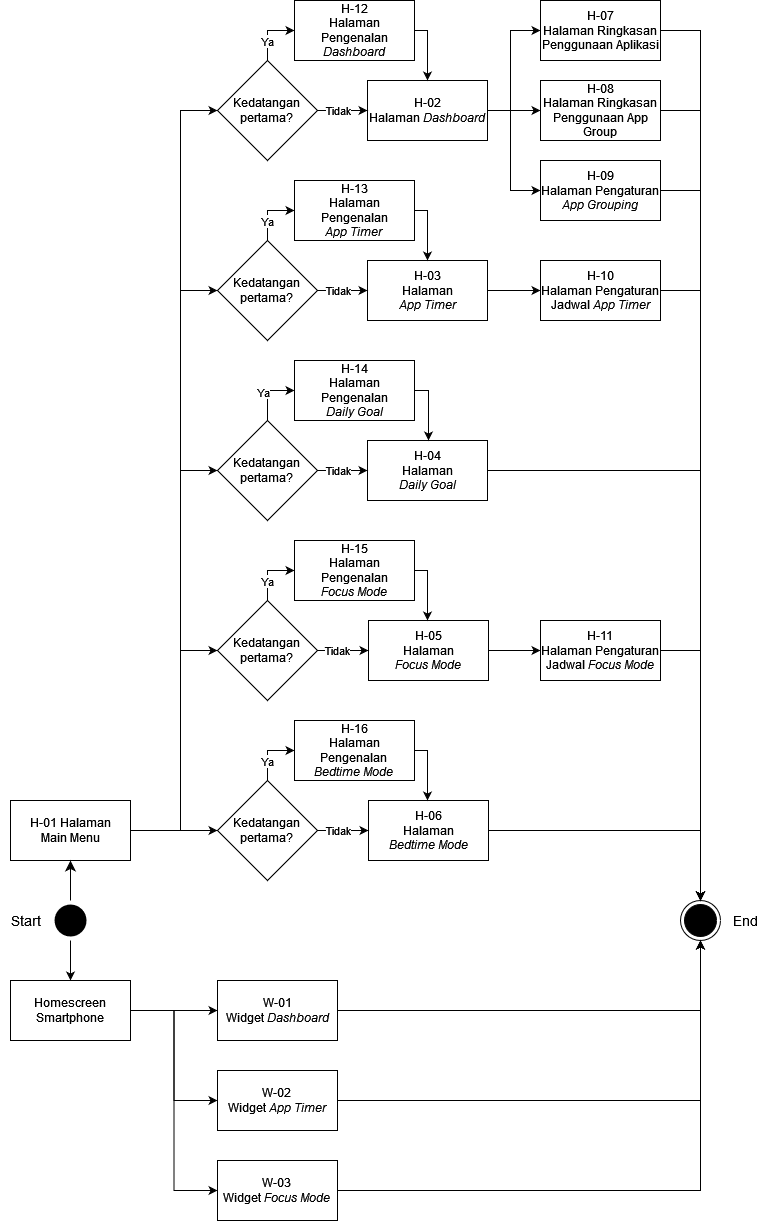
\includegraphics[width=0.68\textwidth]{chapter-3-diagram_user_flow.png}
  \caption{Diagram \textit{User Flow}}
  \label{fig:diagram_user_flow}
\end{figure}
\FloatBarrier

Pengguna dapat memulai \textit{user flow} dari halaman Main Menu, di mana pengguna akan disambut dengan deretan menu menuju 5 halaman utama. Di sini, \textit{user flow} bercabang ke tiap halaman fitur utama, jika pengguna pertama kali masuk ke halaman tersebut maka akan disambut dengan halaman pengenalan tentang fitur yang berkaitan. Berikut adalah penjelasan singkat tentang setiap cabang utama \textit{user flow}

\begin{enumerate}
  \item Saat masuk ke halaman Dashboard, pengguna dapat melihat data penggunaan \textit{smartphone}-nya. Kemudian pengguna dapat melihat detail penggunaan per aplikasi, untuk \textit{app group}, atau menambah \textit{app group} baru.
  \item Saat masuk ke halaman \textit{App Timer}, pengguna dapat melihat daftar aplikasi yang telah dipasangi \textit{App Timer} jika ada. Pengguna juga dapat memasang \textit{App Timer} baru untuk aplikasi lain dengan memilihnya dari daftar aplikasi, di mana pengguna akan masuk ke Halaman Pengaturan Jadwal \textit{App Timer}.
  \item Saat masuk ke halaman \textit{Daily Goal}, pengguna dapat mengatur capaian utama apa yang ingin dijadikan target untuk hari tersebut. Pengguna juga dapat mengatur \textit{Daily Smartphone Evaluation} melalui halaman ini.
  \item Saat masuk ke halaman \textit{Focus Mode}, pengguna dapat melihat jadwal \textit{Focus Mode} yang sedang berlangsung, daftar jadwal \textit{Focus Mode} yang sudah dibuat, serta daftar aplikasi yang dinilai mendistraksi. Pengguna juga dapat mengatur aktivasi \textit{Focus Mode}, serta mengubah atau menambah jadwal \textit{Focus Mode} lewat Halaman Pengaturan Jadwal \textit{Focus Mode}, di mana pengguna juga dapat mengatur kembali aplikasi apa saja yang ingin diblokir selama jadwalnya aktif.
  \item Saat masuk ke halaman \textit{Bedtime Mode}, pengguna langsung dapat mengatur jadwal aktivasi dari \textit{Bedtime Mode}, serta mengatur perilaku dari \textit{Bedtime Mode} sendiri seperti aktivasi \textit{greyscale screen} atau \textit{Do Not Disturb}.
\end{enumerate}

Selain Halaman Main Menu, \textit{user flow} juga dapat dimulai dari Homescreen \textit{smartphone}. Hal ini disebabkan karena \textit{widget} adalah bagian dari aplikasi yang hanya dapat diakses dari Homescreen \textit{smartphone}. \textit{Widget} bertujuan untuk memberikan fungsionalitas atau data dari aplikasi secara lebih cepat dengan tampilan yang lebih sederhana, tanpa memerlukan pengguna untuk mengakses aplikasinya. Maka dari itu, \textit{user flow} untuk \textit{widget} langsung berakhir di \textit{widget} tersebut.

